\documentclass[11pt,a4paper]{article}
\usepackage[margin=25mm]{geometry}
\usepackage[T1]{fontenc}
\usepackage{lmodern}
\usepackage{microtype}
\usepackage{booktabs}
\usepackage{tabularx}
\usepackage{array}
\usepackage{amsmath}
\usepackage{float}
\usepackage{graphicx}
\usepackage{hyperref}
\usepackage{xcolor}
\hypersetup{colorlinks=true,linkcolor=blue!50!black,citecolor=blue!50!black,urlcolor=blue!50!black}
\setlength{\parskip}{0.4em}
\setlength{\parindent}{0pt}
\setlength{\emergencystretch}{2em}
\newcommand{\system}{\textsc{RegulaTrace}}
\newcommand{\field}[1]{\texttt{#1}}
\newcolumntype{Y}{>{\raggedright\arraybackslash}X}
\title{\bfseries RegulaTrace: An Auditable Baseline and Failure Analysis for Regulatory Obligation Extraction}
\author{Lakshit Sachdeva \quad Anannya Samudra\\
Trayee Nayampalli \quad Riddhi Ranjan\\[0.35em]
\small NMIMS MPSTME, Mumbai, India}
\date{27 October 2026\\[0.25em]\small Research preprint draft --- exploratory external evaluation}
\begin{document}
\maketitle
\begin{abstract}
Regulatory obligation analysis requires both correct legal-function decisions and recoverable textual evidence. We present \system, an auditable rule baseline that extracts clause-level modality and fields with source offsets, and compare it with linear text classifiers on two independently released EU datasets. On a five-class deontic-modality proxy (566 distinct texts; three similarity-grouped folds), the rules obtain $0.922\pm0.007$ accuracy and $0.543\pm0.036$ macro F1. On a different regulatory-versus-constitutive task (5,831 distinct sentences from 379 CELEX acts; three act-grouped folds), the same rules obtain $0.419\pm0.070$ accuracy and $0.588\pm0.072$ regulatory-class F1, while a word TF-IDF linear SVM reaches $0.852\pm0.026$ and $0.810\pm0.046$. The contrast is diagnostic: cue recognition works well on explicit modality labels but is nearly non-discriminative when most sentences contain \emph{shall}. A post hoc stress audit further exposes failures in implicit duties, coordinated actions, and inherited context. These exploratory classification results do not measure obligation spans, extracted fields, source authority, or reviewer benefit. We release the evaluation scripts and a separate span-level protocol for that still-needed study.
\end{abstract}
\noindent\textbf{Keywords:} legal NLP; regulatory obligation extraction; deontic modality; provenance; human review; evaluation protocol

\section{Introduction}
An obligation record is only useful if a reviewer can see what the text says, where it says it, and which parts the system inferred. Consider \emph{``The provider must retain logs and notify the authority within 24 hours.''} A single located clause is easy to recover, yet a system that emits one action field has not represented the two coordinated acts separately. Conversely, a perfectly formatted record with the wrong source interval is difficult to audit. These are different errors and require different measurements.

Legal NLP benchmarks establish that evidence and task definitions matter, but they do not make all legal tasks interchangeable. LexGLUE collects legal language-understanding tasks \cite{lexglue}; ContractNLI asks for contract-level inference with supporting spans \cite{contractnli}. Piskorski and Skotarczak extract information-provision requirements from EU legislation, including participants and temporal attributes \cite{piskorski2025}. Minkova et al.\ release deontic-modality labels for EU provisions \cite{minkova2023,minkovadata}; Moodley et al.\ release sentence labels distinguishing regulatory from constitutive statements with CELEX identifiers \cite{moodleydata}. We use the latter two releases for separate, non-interchangeable classification probes of our baseline.

We ask three questions. \emph{RQ1:} How does the rule baseline compare with simple learned models on externally labeled deontic modality? \emph{RQ2:} Does that result persist when the task is to distinguish regulatory obligations from constitutive statements? \emph{RQ3:} Which evidence and representation failures remain outside both classification tasks? We answer the first two with measured, reproducible proxy experiments and the third with a source-offset contract and stress audit. The 16-case development suite remains a software check, not the principal empirical result.

\section{Position Among Related Tasks}
\begin{table}[ht]
\centering\small
\caption{Nearby research tasks and the difference in prediction target. This table compares task formulations, not system scores.}
\label{tab:related}
\begin{tabularx}{\linewidth}{@{}p{0.22\linewidth}Y Y@{}}
\toprule
Work & Primary target & Relationship to this study\\
\midrule
LexGLUE \cite{lexglue} & Multiple legal understanding tasks & Demonstrates task-specific evaluation; no common obligation-record target.\\
ContractNLI \cite{contractnli} & Contract-level inference with evidence spans & Motivates evidence location, but its labels and document questions differ.\\
Minkova et al.\ \cite{minkova2023} & Deontic modality in EU legislation & Closest to the modality subtask; does not by itself validate our actor, action, or provenance fields.\\
Piskorski and Skotarczak \cite{piskorski2025} & Information-provision activities and attributes & Closest regulatory extraction setting; different corpus and output schema.\\
Moodley et al.\ \cite{moodleydata} & Regulatory versus constitutive EU statements & Tests legal function when modal words alone are insufficient; no obligation span labels.\\
\bottomrule
\end{tabularx}
\end{table}

\section{Task and Evidence Contract}
Let a document be a Unicode string $T$ with a source identifier and version metadata. The current system segments $T$ into candidate clauses. For each clause, it proposes a record
\[
r=(m,a,x,d,c,e,q,[b,u),v),
\]
where $m$ is modality, $a$ actor, $x$ action, $d$ raw deadline expression, $c$ condition, $e$ exception, $q$ quoted evidence, $[b,u)$ a source interval, and $v$ source version. Offsets count Unicode code points; $u$ is exclusive. The operational labels are obligation, prohibition, recommendation, permission, and information. The information label routes descriptive or epistemic statements away from the normative register.

A located record must be checkable against the supplied or extracted text: the interval $T[b:u]$ should recover the retained clause after whitespace normalization. The identifier and evidence quote do not prove that an uploaded document is an authoritative legal source. PDF offsets refer to extracted text, not page coordinates. Cross-references are recorded but are not automatically resolved; fields that require surrounding provisions can remain unresolved.

We distinguish three properties that are often conflated. \emph{Offset validity} asks whether $0\leq b<u\leq |T|$ and the interval reconstructs the saved evidence. \emph{Candidate correctness} asks whether that interval expresses a normative act. \emph{Field correctness} asks whether the actor, action, timing, and exceptions preserve the rule's meaning. Offset validity can be checked automatically against $T$; the latter two require independent annotation. A system can satisfy the first while failing the others, as the coordinated-action example in Section~\ref{sec:diagnostic} shows.

The baseline's unit is one record per segmented clause. The proposed evaluation unit is one annotated normative span per duty. These units need not coincide. A sentence with two acts may yield one baseline record but two gold duties; conversely, a duty that inherits a condition from another sentence may need a wider interpretive context than the baseline stores. The evaluation protocol makes this mismatch visible instead of treating a located clause as a complete obligation.

\begin{figure}[t]
\centering
\fbox{\begin{minipage}{0.91\linewidth}\centering
\textbf{Supplied text and metadata}\\[0.35em]
$\downarrow$ clause segmentation and source-offset location\\[0.35em]
\textbf{Modality and heuristic field extraction}\\[0.35em]
$\downarrow$ typed obligation record with evidence and unresolved flags\\[0.35em]
\textbf{Policy and version triage}\quad $\longrightarrow$\quad \textbf{Reviewer decision and audit event}
\end{minipage}}
\caption{Implemented local pipeline. The policy and version branches provide review signals; they do not issue legal compliance determinations.}
\label{fig:pipeline}
\end{figure}

\section{Implemented Baseline}
\subsection{Ingestion and obligation extraction}
The FastAPI application accepts text-based PDF, DOCX, TXT, and Markdown. Scanned PDFs require OCR outside the present pipeline. Clause segmentation uses punctuation, line boundaries, and list markers. Ordered patterns identify modal cues such as \emph{must}, \emph{shall not}, \emph{should}, and \emph{may}; a special rule treats phrases such as \emph{may not be complete} as epistemic information rather than prohibition. Actor and action are derived from text around the cue. Further patterns identify raw deadlines, conditions, exceptions, and cross-references. The action parser strips certain leading timing qualifiers before selecting the operative phrase; this addresses a failure exposed by the bundled breach-notification example.

The source locator searches clauses in document order and returns exact start and end offsets when a normalized clause can be found. It returns a missing value and an unresolved flag when it cannot locate one. The implementation maintains corresponding Python and browser JavaScript engines. Its numerical confidence is a hand-built heuristic based on cues and completeness, not a calibrated probability.

Ordered cue matching imposes a strong inductive bias: explicit prohibitions take precedence over obligations, followed by recommendations and permissions; clauses with no recognized cue become information. The special epistemic rule for phrases such as \emph{may not be complete} prevents one obvious false prohibition. It cannot infer that \emph{is under a duty to} expresses an obligation. Actor extraction uses text before the cue and action extraction uses text after it. The rule is transparent, but it is sensitive to intervening parentheticals, coordination, and antecedents in earlier clauses.

\subsection{Policy comparison and version triage}
The current policy comparator reads the first extracted requirement and policy records, then scores actor, action, polarity, timing, exception, and evidence dimensions. Lexical overlap and approximate numeric time conversion feed a weighted score, with polarity and timing failures able to override an otherwise high score. The output is \emph{likely aligned}, \emph{review required}, or \emph{potential mismatch}. It is not a legal conclusion, and it does not implement corpus retrieval or semantic entailment.

Version triage greedily aligns old and new clauses by token overlap. It reports added, removed, and modified clauses, followed by a severity signal and a text-based change explanation. A proposed reason is labeled as an inference; legislative intent cannot be established from two text versions alone. Reordered clauses, inherited context, paraphrases, and definition changes remain difficult for this alignment method.

\subsection{Human review and local audit}
The application stores analyses and review events in local SQLite. A reviewer can confirm, reject, or correct selected fields. A correction updates the saved record and records before/after values, reviewer, note, and timestamp while retaining the original evidence clause. The UI can reopen a saved case and show its current review state. This is a single-user local workflow without identity management or role-based access.

The review log preserves the distinction between a model proposal and a human correction. It does not establish that a correction is legally correct; that would require an adjudication procedure and an authoritative source. Nor is the number of corrections a performance metric without a controlled review design: reviewers may focus on visibly uncertain records and ignore silent omissions.

\section{Evaluation Design}
\subsection{Synthetic development checks}
The repository contains a transparent challenge suite: 12 extraction cases, three policy-comparison cases, and one version-change case. Extraction checks include modality, actor, deadline when present, and evidence location. Nine cases are designated critical for the safety diagnostic. We define a \emph{critical miss} as a materially misread or missed duty in those extraction cases, a missed serious policy mismatch, or a missed material version change. This denominator differs from the overall pass rate. The examples were authored with the system and are not an independent sample from legal practice.

\subsection{External classification probes}
We run two \emph{exploratory proxy tasks}, with their labels and scripts kept separate. The first uses Minkova et al.'s released EU deontic-modality CSV \cite{minkovadata}. We retain only annotator A1's 567 labeled rows, remove one same-label duplicate after trimming surrounding whitespace, and evaluate 566 distinct texts: 444 obligations, 83 permissions, 17 prohibitions, 9 powers, and 13 rights. The separate unannotated \field{None} rows are excluded. Because document IDs are absent, we group texts with character 3--5-gram TF-IDF cosine similarity at least 0.75 before three-fold stratified cross-validation (551 groups; seed 42). This reduces obvious near-duplicate leakage but cannot guarantee document-level independence.

The second uses the human-labeled regulatory-versus-constitutive sentence release of Moodley et al.\ \cite{moodleydata}. From 7,240 CSV rows, we require a sentence, a CELEX identifier, and a binary label; normalize whitespace; deduplicate identical text; and exclude 269 exact-text groups with discordant labels. The retained 5,831 sentences come from 379 CELEX acts and comprise 2,494 regulatory and 3,337 constitutive labels. All sentences with the same CELEX act remain in one of three stratified folds (seed 42). Nearly all retained sentences (5,776/5,831) contain \emph{shall}; this is a difficult setting for modal-cue rules, not a representative prevalence sample of all EU sentences.

We compare the existing \system\ engine, a majority-class predictor, word unigram/bigram TF-IDF with logistic regression, word TF-IDF with linear SVM, and character 3--5-gram TF-IDF with linear SVM. Vectorizers are fitted within each training fold. Model hyperparameters, source file hashes, cleaning rules, and library versions are recorded in the released scripts and result JSON. In the deontic task, the engine's first normative record provides a label; its unsupported \emph{power} and \emph{right} classes, and any information or recommendation output, count as errors. In the binary task, any normative record maps to \emph{regulatory}. These mappings are intentionally simple and do not transform the engine into a trained classifier.

We report mean accuracy and task-specific F1 across the three folds with one fold standard deviation, not a confidence interval. Five-class macro F1 gives each deontic label equal weight. Binary F1 treats \emph{regulatory} as positive; precision and recall are computed from pooled out-of-fold predictions. This study was designed after inspecting the available datasets and has no preregistered model selection. It is not a direct comparison to scores in the source papers, which used different splits and preprocessing.

\subsection{Held-out document protocol}
A separate, still-unpopulated JSON Lines format specifies one document per row, including document ID, source-group ID, split, text, and zero or more annotated normative spans with modality and a preassigned critical flag. A descriptive-only document has an empty annotation list. The loader rejects malformed offsets, overlapping gold spans, repeated document IDs, and source or exact-text leakage across train, development, and test splits. Near duplicates still require manual review. Two annotators should independently label test documents and adjudicate disagreements without seeing predictions.

The evaluator matches predicted and gold spans one to one by descending character intersection-over-union, with a prespecified threshold of 0.5. Unmatched gold spans are false negatives and unmatched predictions are false positives. It reports precision, recall, and F1 for candidate detection; modality accuracy on matched spans; and
\[
\mathrm{CMR}=\frac{\#\{\text{critical gold duties unmatched or wrong modality}\}}
{\#\{\text{critical gold duties}\}}.
\]
When there are no critical gold duties, CMR is undefined and is reported as null. The evaluator also checks whether each predicted evidence interval maps back to the supplied text and emits error rows for review. The report includes the engine version, split, raw counts, and a hash of the selected documents.

\subsection{Analysis plan and validity checks}
The primary independent outcome should be critical-duty miss rate on a frozen test set, reported with its numerator and denominator. Candidate precision, recall, and F1 are necessary secondary outcomes because a system can reduce misses by flooding reviewers with false positives. Modality accuracy is conditional on a matched span and must not be read as overall classification accuracy. Provenance validity is an engineering invariant, not a proxy for legal correctness. For each metric, report document-level uncertainty intervals and per-source breakdowns where counts permit; do not tune a threshold after reading the test errors.

Annotation quality is itself a measurement problem. The initial study should pilot at least 20 diverse source documents to refine the unit of annotation, including coordinated duties, exceptions, cross-references, and descriptive controls. This is a planned pilot size, not an existing corpus. Two annotators should then label test documents independently, record span overlap and modality agreement before adjudication, and resolve disagreements without model output. Related sections and versions of the same instrument must share a source-group ID. Exact-text leakage is rejected by code; near-duplicate versions still need manual review. A comparison with learned models is only interpretable if every model receives the same text and emits the same span-and-modality contract.

A separate reviewer study would test practical value. Reviewers should receive randomly assigned cases with or without system suggestions, use a shared answer key established independently, and record time, accepted errors, missed duties, and correction effort. This prospective design is distinct from offline extraction scoring; a correction log from ordinary use cannot establish a causal time benefit.

\begin{table}[H]
\centering
\caption{Current executable checks. These are development and engineering checks, not held-out estimates.}
\label{tab:checks}
\begin{tabularx}{\linewidth}{@{}YrrY@{}}
\toprule
Check & Cases & Passed & Interpretation\\
\midrule
Synthetic extraction & 12 & 12 & Cue, actor, timing, and provenance checks\\
Synthetic policy comparison & 3 & 3 & Expected triage outcome\\
Synthetic version change & 1 & 1 & Added and modified clauses detected\\
Critical subset & 9 & 9 & Zero misses on selected synthetic cases\\
\bottomrule
\end{tabularx}
\end{table}

\section{Observed Checks and Diagnostic Failure Audit}\label{sec:diagnostic}
\subsection{What the development suite establishes}
Table~\ref{tab:checks} reports the executable suite at the code snapshot used for this draft. All 16 cases pass, including nine marked critical by the suite authors. Most extraction cases are single, explicit modal sentences. They test whether the code recognizes those cues, selected actor and timing fragments, and an exact evidence span. The critical subset is not a randomly sampled set of high-consequence duties. A fictional demonstration DOCX produced 30 segmented records with 30 located source intervals, and local verification passed 20 Python and eight JavaScript tests. These observations establish that the program runs on the listed fixtures and that its evidence and review contracts are testable. They do not estimate precision, recall, or analyst benefit on real regulations.

\subsection{Five-class deontic modality proxy}
Table~\ref{tab:deontic-results} and Figure~\ref{fig:deontic-scores} report measured cross-validation results. The rule baseline has the highest mean accuracy ($0.922$) and macro F1 ($0.543$) among these fixed comparators. The strongest learned macro F1 is $0.499$ for word TF-IDF with logistic regression. This is evidence that the released sample's explicit cues are well matched to the rules, not evidence that the full structured obligation record is correct. The majority classifier's $0.784$ accuracy and $0.176$ macro F1 show why accuracy alone is weak under the class imbalance.

\begin{table}[H]
\centering\small
\caption{Deontic-modality proxy: mean $\pm$ one fold SD across three similarity-grouped folds ($n=566$). Scores are fractions.}
\label{tab:deontic-results}
\begin{tabularx}{\linewidth}{@{}Ycc@{}}
\toprule
Model & Accuracy & Macro F1\\
\midrule
\system\ rules & $0.922\pm0.007$ & $0.543\pm0.036$\\
Majority class & $0.784\pm0.044$ & $0.176\pm0.006$\\
Word TF-IDF + logistic regression & $0.866\pm0.038$ & $0.499\pm0.060$\\
Word TF-IDF + linear SVM & $0.878\pm0.041$ & $0.487\pm0.115$\\
Character TF-IDF + linear SVM & $0.855\pm0.044$ & $0.377\pm0.073$\\
\bottomrule
\end{tabularx}
\end{table}

\begin{figure}[H]
\centering
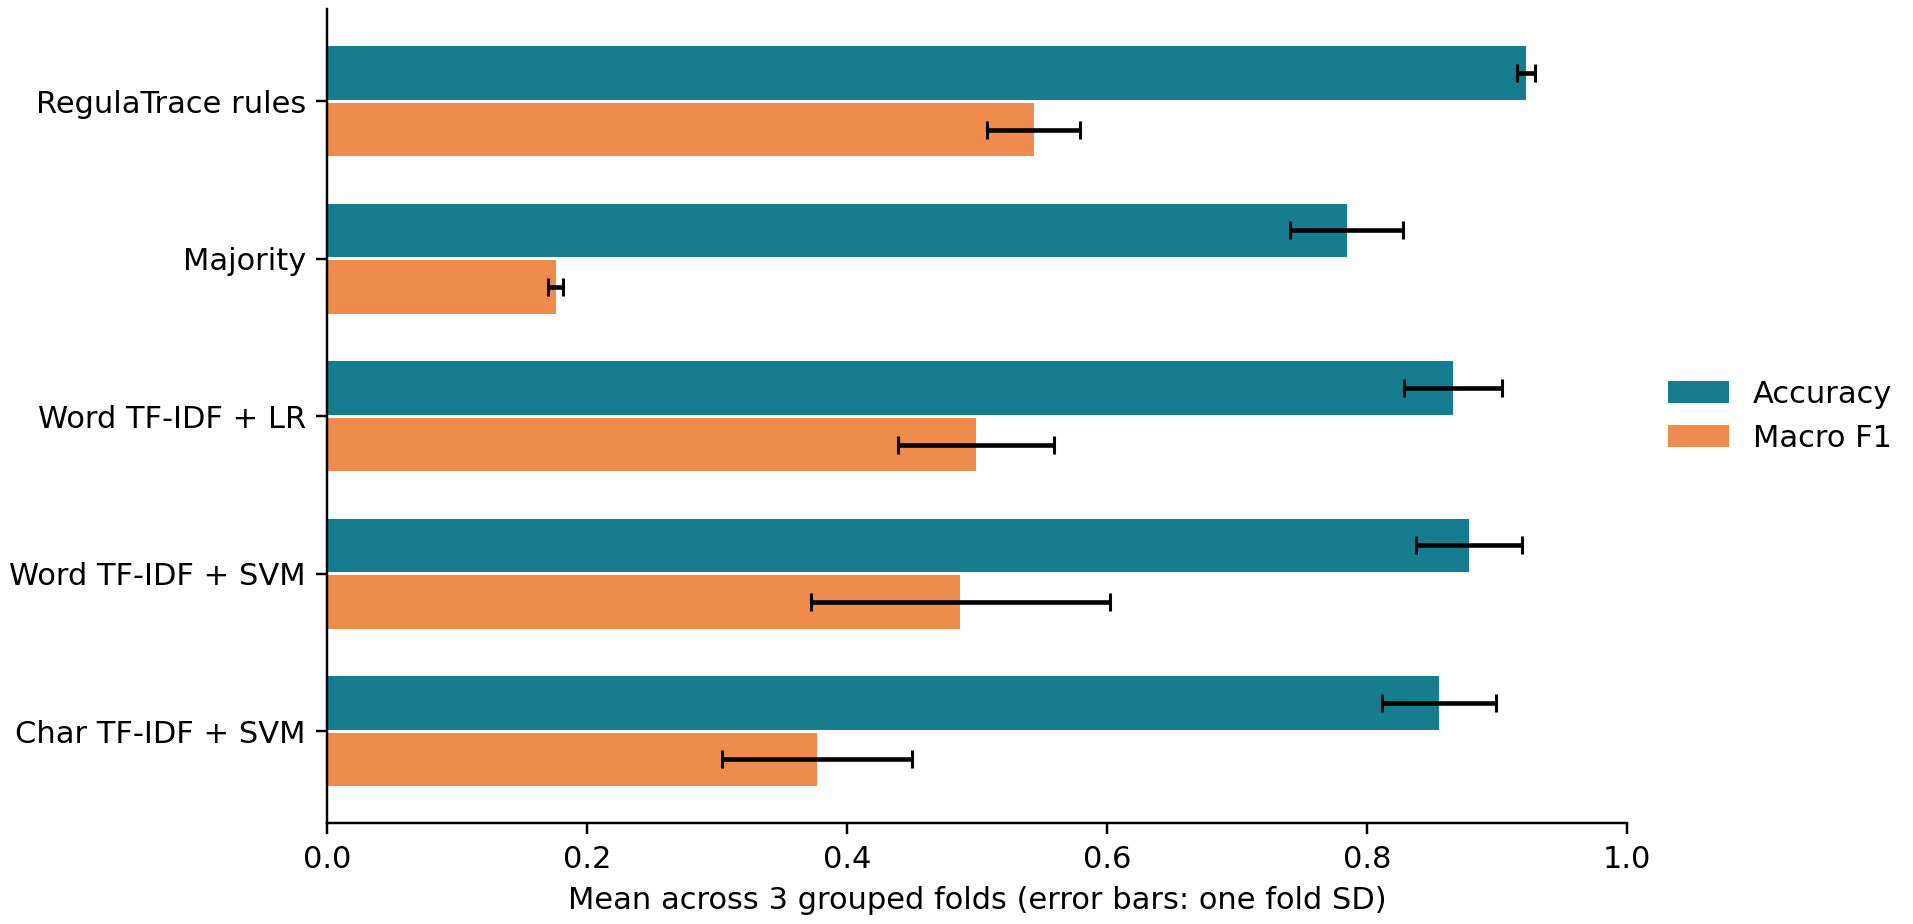
\includegraphics[width=0.95\linewidth]{figures/deontic_proxy_scores.png}
\caption{Accuracy and macro F1 on the five-class modality proxy. Error bars are one fold standard deviation; they are not confidence intervals.}
\label{fig:deontic-scores}
\end{figure}

The aggregate hides a hard label-space boundary. Figure~\ref{fig:deontic-perclass} shows out-of-fold F1 by class. \system\ obtains approximately $0.97$, $0.90$, and $0.88$ F1 for obligation, permission, and prohibition, but $0$ for power and right because its output vocabulary has neither class. These latter classes have only 9 and 13 examples, so even learned-model estimates are unstable. The rule engine also abstains on 17 texts; its five-class evaluation counts every abstention as an error.

\begin{figure}[H]
\centering
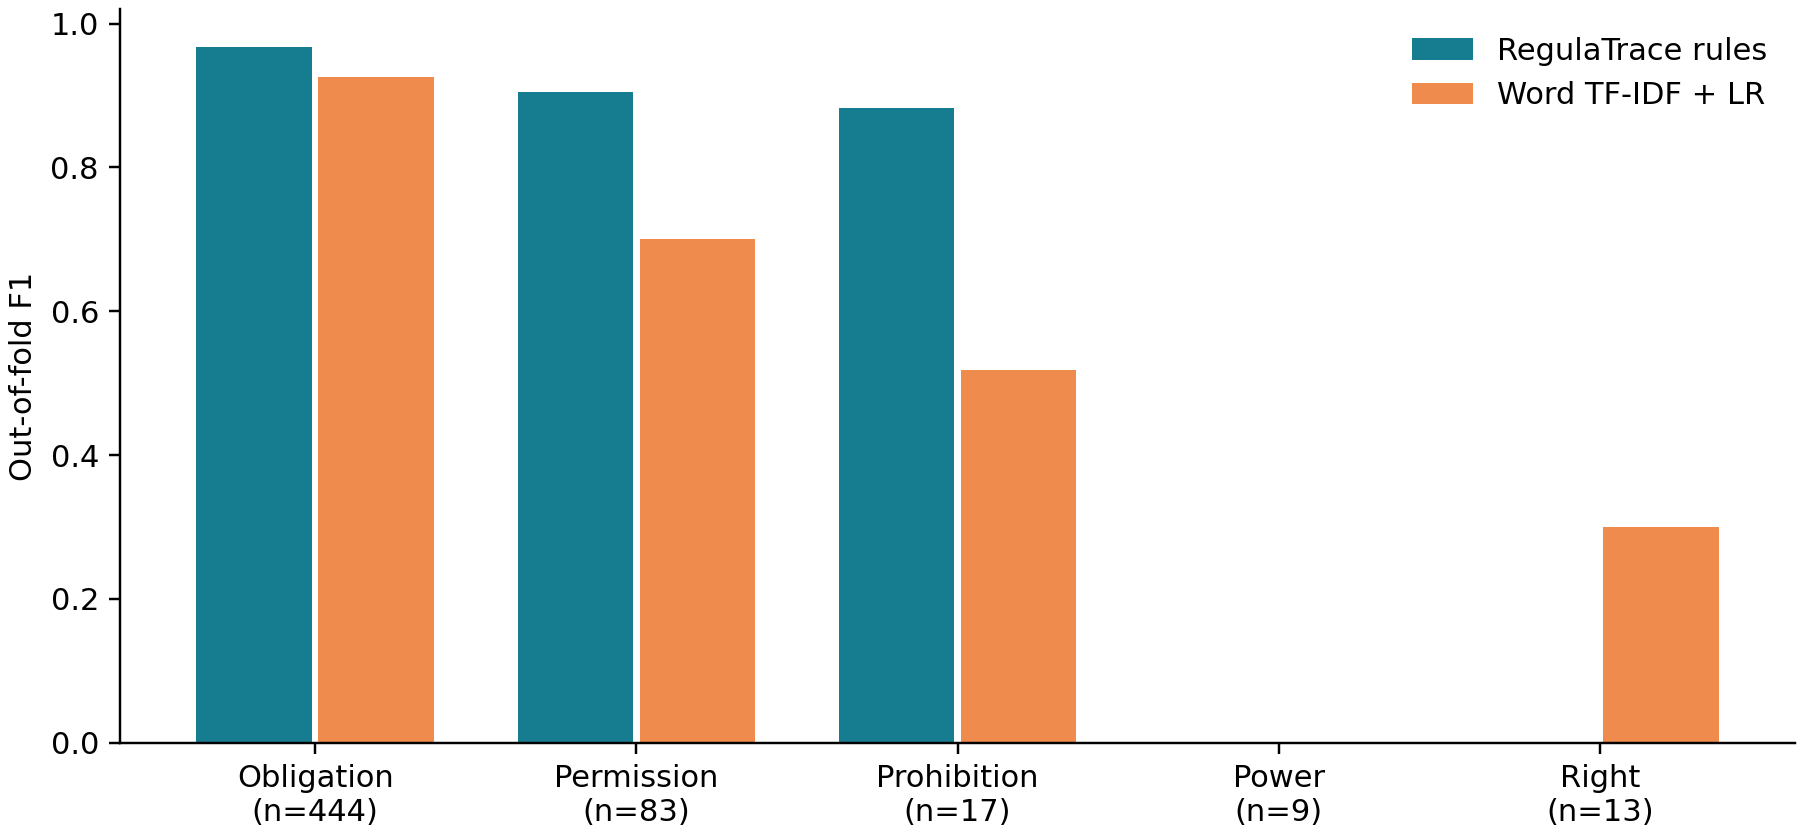
\includegraphics[width=0.88\linewidth]{figures/deontic_proxy_per_class.png}
\caption{Pooled out-of-fold F1 by gold deontic class; $n$ gives class support. Word logistic regression is the strongest learned comparator by mean macro F1.}
\label{fig:deontic-perclass}
\end{figure}

\subsection{Regulatory versus constitutive statements}
The result reverses on the second task (Table~\ref{tab:binary-results}, Figure~\ref{fig:binary-scores}). Here \system\ achieves $0.419$ mean accuracy and $0.588$ regulatory-class F1, whereas the word TF-IDF SVM reaches $0.852$ and $0.810$. The majority classifier reaches $0.581$ accuracy but zero positive-class F1. The different denominators and labels mean the two tables must not be interpreted as a single benchmark ranking.

\begin{table}[H]
\centering\small
\caption{Regulatory-versus-constitutive task: mean $\pm$ one fold SD across three CELEX-grouped folds ($n=5{,}831$). Positive-class F1 treats regulatory as positive.}
\label{tab:binary-results}
\begin{tabularx}{\linewidth}{@{}Ycc@{}}
\toprule
Model & Accuracy & Regulatory F1\\
\midrule
\system\ rules & $0.419\pm0.070$ & $0.588\pm0.072$\\
Majority class & $0.581\pm0.071$ & $0.000\pm0.000$\\
Word TF-IDF + logistic regression & $0.834\pm0.027$ & $0.779\pm0.040$\\
Word TF-IDF + linear SVM & $0.852\pm0.026$ & $0.810\pm0.046$\\
Character TF-IDF + linear SVM & $0.829\pm0.026$ & $0.780\pm0.057$\\
\bottomrule
\end{tabularx}
\end{table}

\begin{figure}[H]
\centering
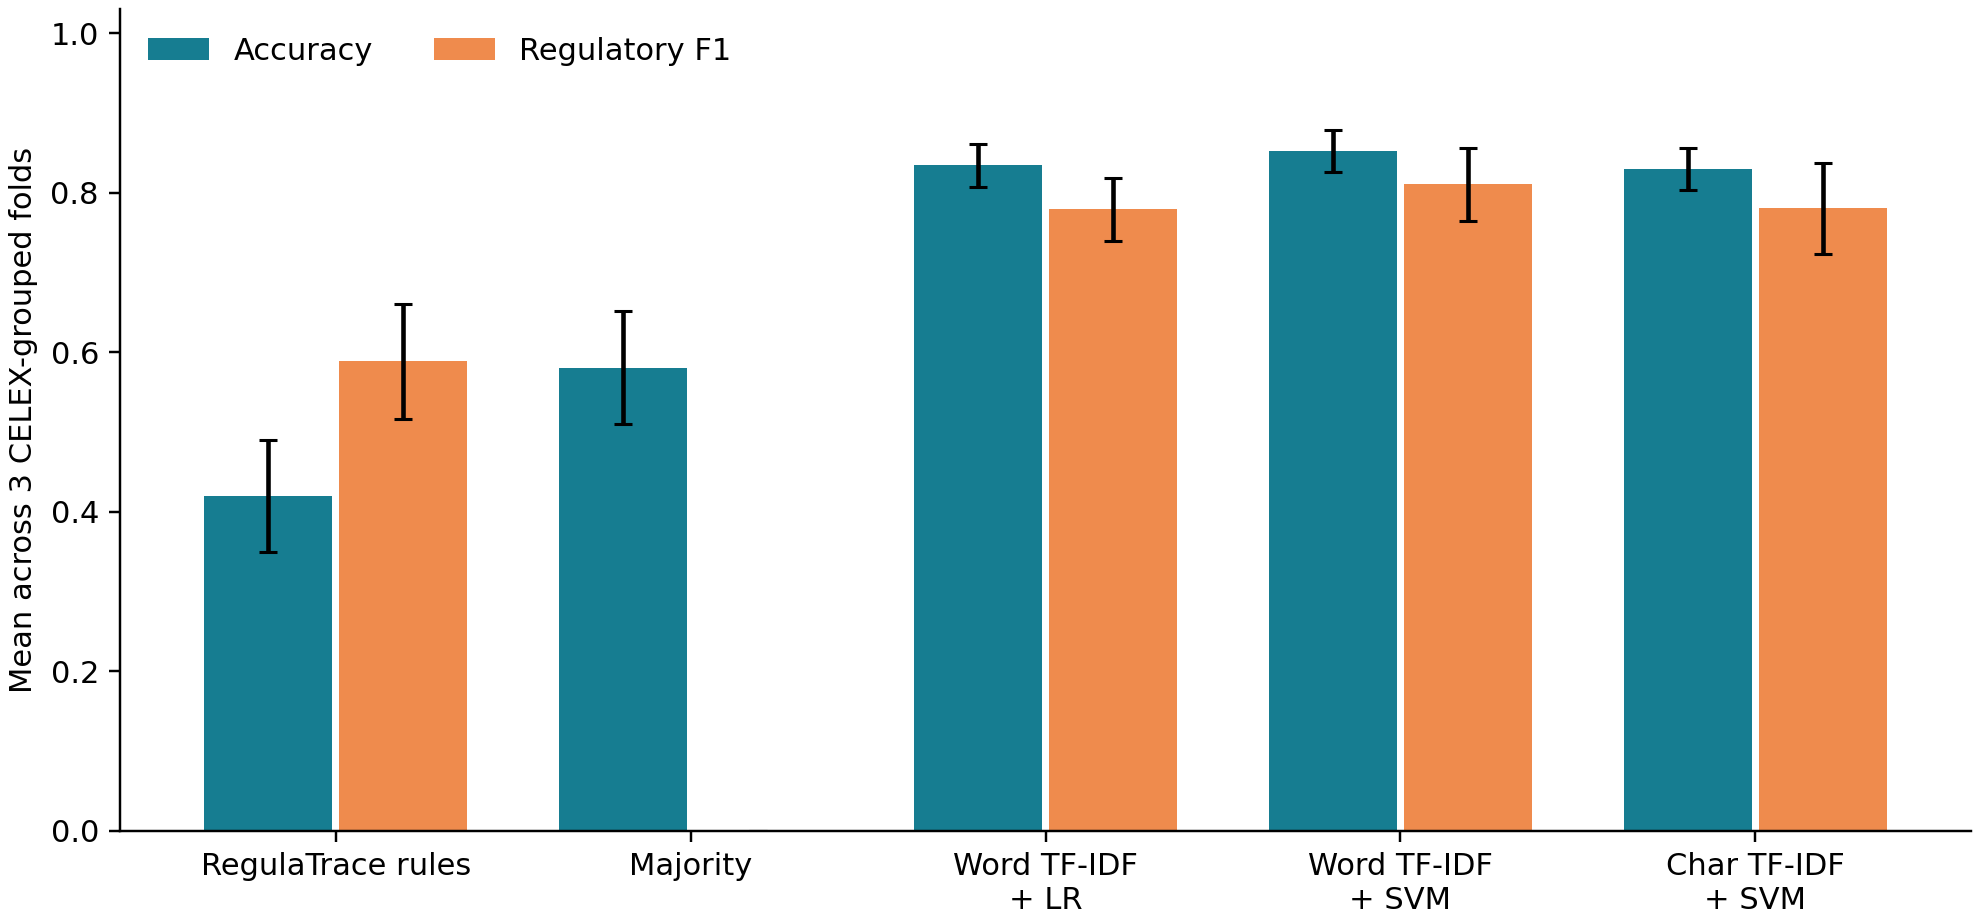
\includegraphics[width=0.95\linewidth]{figures/regulatory_binary_scores.png}
\caption{External regulatory-versus-constitutive classification. Error bars are one fold standard deviation; source acts, not individual sentences, define folds.}
\label{fig:binary-scores}
\end{figure}

Figure~\ref{fig:binary-confusion} explains the rule baseline's poor accuracy. In pooled out-of-fold predictions it detects all 2,494 regulatory sentences, but it also calls 3,336 of 3,337 constitutive sentences regulatory: recall is $1.000$, precision is $0.428$, and specificity is approximately $0.0003$. The word SVM instead has 1,924 true positives, 298 false positives, and 570 false negatives (precision $0.866$, recall $0.771$). This is a real trade-off: the learned model sharply reduces false alarms but misses some positive examples. The near-constant presence of \emph{shall} makes a modal cue almost useless for this particular binary distinction.

\begin{figure}[H]
\centering
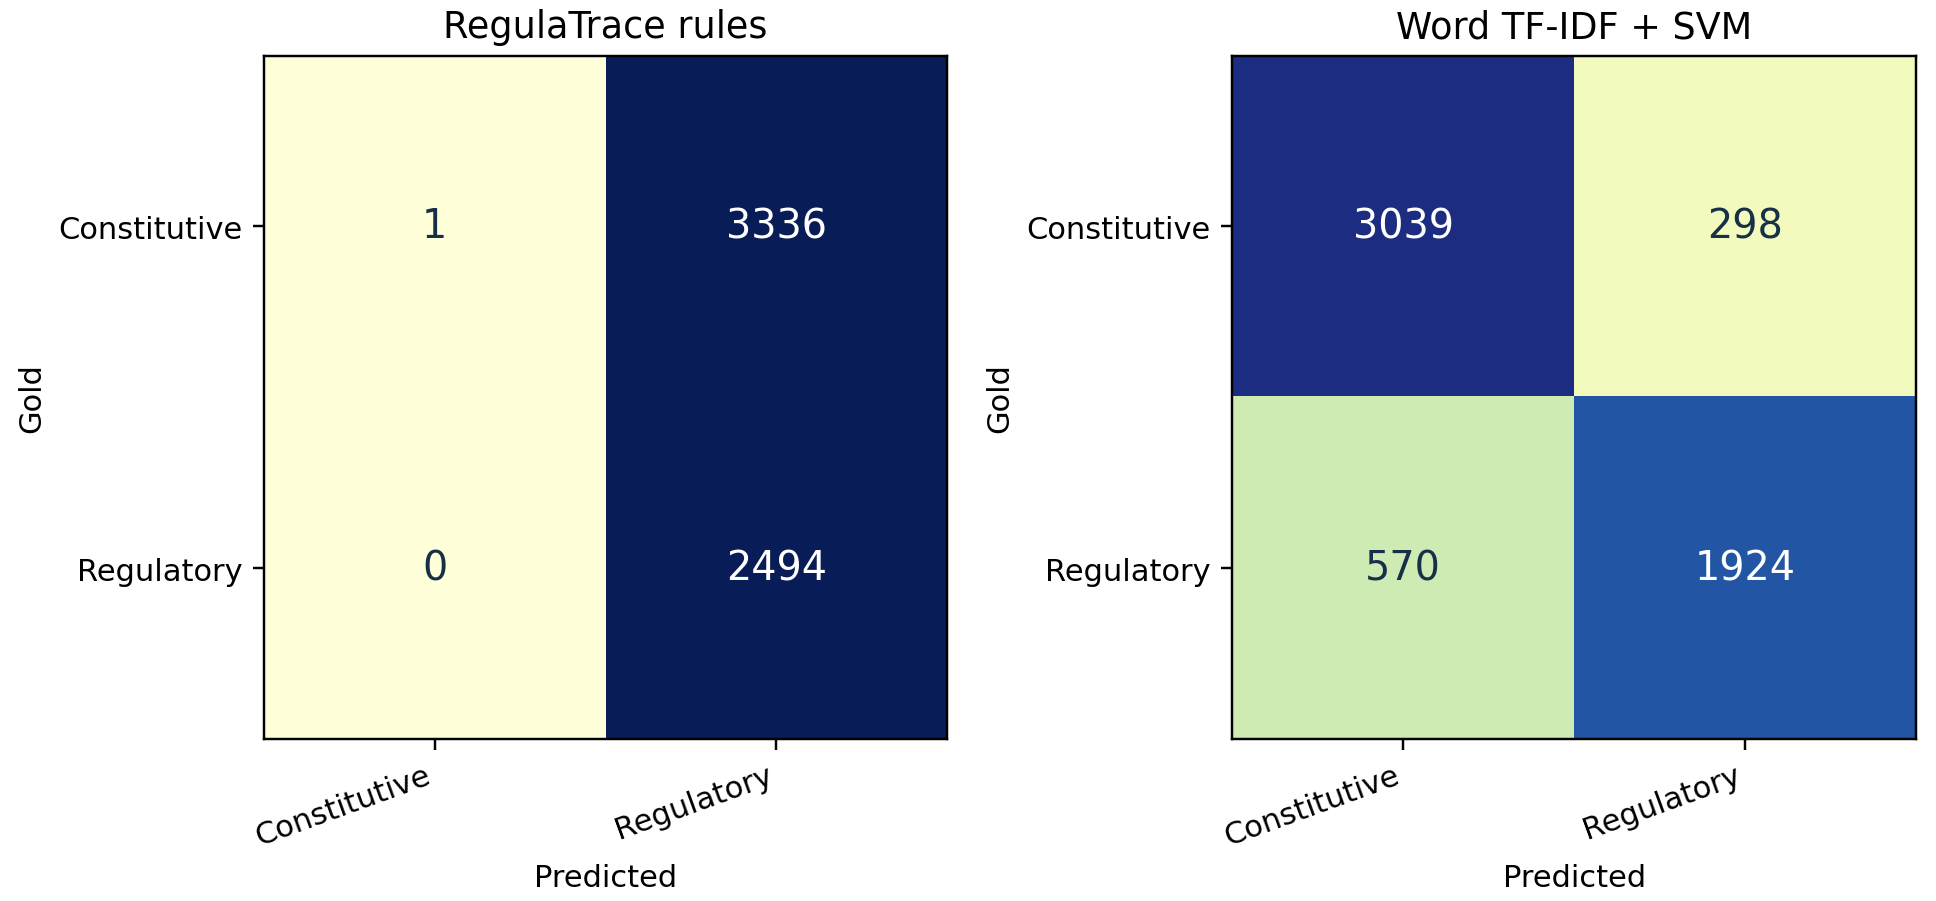
\includegraphics[width=0.92\linewidth]{figures/regulatory_binary_confusion.png}
\caption{Pooled out-of-fold confusion counts. Cell shading is normalized within each gold row, so rare errors remain visible; numbers are unnormalized counts.}
\label{fig:binary-confusion}
\end{figure}

\subsection{Post hoc stress audit}
After inspecting the baseline, we constructed short, fictional clauses to probe representational limits. This is a qualitative diagnostic exercise: the prompts are neither independently sampled nor blinded, and no aggregate accuracy is reported. Table~\ref{tab:stress} records actual Python-engine behavior. The inputs and observed fields are short enough to reproduce with \field{backend.engine.analyze\_document}; the table reports failures rather than hiding them in a single pass rate.

\begin{table}[ht]
\centering\footnotesize
\caption{Selected post hoc stress probes and observed behavior. All inputs are fictional; these are examples of failure mechanisms, not prevalence estimates.}
\label{tab:stress}
\begin{tabularx}{\linewidth}{@{}p{0.23\linewidth}Y Y@{}}
\toprule
Construction & Input excerpt & Observed behavior\\
\midrule
Implicit modality & ``The licensee is under a duty to maintain records.'' & Classified as information; zero normative records.\\
Coordinated acts & ``The provider must retain logs and notify the authority within 24 hours.'' & One obligation record; action joins both acts, so separate responsibilities are unavailable.\\
Anaphoric actor & ``The controller must secure records. It must also notify the authority.'' & Two obligations; second actor is literally ``It,'' without antecedent resolution.\\
Interrupted modal phrase & ``Every provider must, unless exempt, keep records.'' & Obligation cue found, but action is unresolved and exception absorbs ``keep records.''\\
Elliptical coordination & ``The operator shall retain logs for 30 days; and delete them after this period.'' & First clause is normative; the deletion clause is classified as information.\\
Multiple time expressions & ``All licensees are required to report incidents within 24 hours and retain evidence for 5 years.'' & One record and one extracted deadline (``within 24 hours''); retention duration is not represented separately.\\
\bottomrule
\end{tabularx}
\end{table}

These cases expose a methodological issue, not just missing regexes. A clause-level record with one actor, one action, and one deadline cannot faithfully represent multiple duties without splitting or a richer relation structure. The anaphora example also shows that a nonempty actor field is weaker than a resolved actor. The exception example shows that evidence location may remain valid while the extracted action and exception are wrong. Thus an offset-only provenance score would overstate semantic reliability.

The audit also included two useful positive controls. \emph{``Records may not be complete when the migration begins''} was routed to information rather than misread as a prohibition. \emph{``If a breach occurs, the controller must notify the authority unless the risk is negligible''} yielded an obligation with the actor, condition, and exception separated as intended. Their success does not cancel the failures above; it identifies which local constructions the present rules handle.

\subsection{What remains to be measured}
The external datasets support sentence-level classification claims only. Neither provides the gold obligation spans, actor/action fields, linked exceptions, source-offset judgments, or reviewer decisions needed to evaluate the full \system\ record. The first dataset lacks act IDs, and its rare classes create high variance; similarity groups cannot prove source independence. The second has CELEX groups, but excluding discordant text groups may alter its label distribution, and its regulatory label is narrower than the engine's any-normative decision. Model families and preprocessing were selected during this exploratory study, so the best observed result is not a confirmatory generalization estimate.

A future end-to-end study should pilot the annotation guide on diverse sources, freeze a source-disjoint test set, and compare rules with a character n-gram linear model, a general encoder, and a legal-domain encoder such as LEGAL-BERT \cite{legalbert} under the same span-and-field output contract. The literature cautions against assuming a larger model will dominate simple baselines on every legal extraction task \cite{piskorski2025}. Field-level span F1, change-impact recall, policy-outcome macro F1, calibrated uncertainty, and reviewer time require additional gold labels and prospective designs; this paper reports none of them.

\section{Limitations, Ethics, and Reproducibility}
The stress audit points to four distinct error sources. \emph{Coverage error:} implicit duties and elliptical follow-on clauses can be assigned to information. \emph{Unit error:} coordinated acts are compressed into one record. \emph{Context error:} pronouns, inherited actors, and cross-references are not resolved. \emph{Field error:} interruptions such as an exception between modal and verb can contaminate the action and exception strings. The baseline favors explicit English modal language and has not been evaluated for tables, OCR noise, multilingual regulations, or duties distributed across provisions. Clause-level evidence is narrower than field-level evidence: actor, action, and deadline strings are not individually span-validated.

Greedy version matching and first-record policy comparison may fail on multi-clause documents. Approximate time conversion omits legal calendars and trigger semantics. Confidence is heuristic and uncalibrated; the numbers should not be interpreted as error probabilities. A missing source interval is surfaced, but a present interval alone does not establish source authority, correct interpretation, or compliance. The current diagnostic examples were selected after code inspection and can reveal possible failures, not their frequency in a target population.

Regulatory text can guide consequential work. The interface therefore presents its outputs as review signals, preserves corrections, and avoids an automatic compliance certification claim. The local store is not designed for confidential multi-user deployment. Any future human study should obtain appropriate permissions, avoid collecting unnecessary personal data, and disclose whether reviewers saw system suggestions.

The implementation snapshot and synthetic suite are available through the public \system\ repository and draft research branch at commit \field{9ae8ae8}.\footnote{\href{https://github.com/trayee05/regulatrace-compliance-intelligence}{Source repository}; \href{https://github.com/lakshitsachdeva/regulatrace-compliance-intelligence/commit/9ae8ae87a1890363690a37d448dd5f7cc18c9e3b}{implementation snapshot}.} The experimental scripts, source-file hashes, cleaning rules, fold metrics, and plot generation are in \field{research/experiments/}; the released datasets are downloaded from their cited repositories and are not redistributed here. The span-level evaluator and annotation rules are in \field{research/}. No annotated end-to-end obligation-record corpus is released with this draft. The system uses exact source offsets within the supplied text but does not verify official source identity or PDF page coordinates.

\section{Conclusion}
\system\ demonstrates that recoverable evidence, inspectable rules, and a persistent correction trail can be implemented together. On one external modality proxy, its cue rules are competitive with fixed linear baselines; on a second, source-grouped regulatory-function task they overpredict almost every sentence, while a word SVM markedly reduces false positives at the cost of some misses. Both results are exploratory sentence-classification measurements. The post hoc stress audit adds a separate representational warning: one record per clause cannot reliably express multiple, inherited, or context-dependent duties. A source-disjoint, independently annotated span-and-field study is still required before claiming end-to-end obligation extraction quality or reviewer benefit.

\begin{thebibliography}{9}
\bibitem{lexglue}
I. Chalkidis, A. Jana, D. Hartung, M. Bommarito, I. Androutsopoulos, D. Katz, and N. Aletras.
LexGLUE: A benchmark dataset for legal language understanding in English.
In \emph{Proceedings of ACL}, pages 4310--4330, 2022.
\href{https://doi.org/10.18653/v1/2022.acl-long.297}{doi:10.18653/v1/2022.acl-long.297}.

\bibitem{contractnli}
Y. Koreeda and C. D. Manning.
ContractNLI: A dataset for document-level natural language inference for contracts.
In \emph{Findings of EMNLP}, pages 1907--1919, 2021.
\href{https://doi.org/10.18653/v1/2021.findings-emnlp.164}{doi:10.18653/v1/2021.findings-emnlp.164}.

\bibitem{minkova2023}
K. Minkova, S. M. Chakravarthy, and G. van Dijck.
Low-resource deontic modality classification in EU legislation.
In \emph{Proceedings of NLLP}, 2023.
\url{https://aclanthology.org/2023.nllp-1.15/}.

\bibitem{minkovadata}
K. Minkova, S. M. Chakravarthy, and G. van Dijck.
Low-resource deontic modality classification in the EU legislation: released dataset.
DataverseNL, 2024.
\href{https://doi.org/10.34894/HQ8LIH}{doi:10.34894/HQ8LIH}.

\bibitem{moodleydata}
K. Moodley, G. J. Brandsma, J. Blom-Hansen, and C. Meijer.
Reproducibility data for a study of regulatory statements in EU legislation.
Zenodo, 2023.
\href{https://doi.org/10.5281/zenodo.8200001}{doi:10.5281/zenodo.8200001}.

\bibitem{piskorski2025}
J. Piskorski and D. Skotarczak.
Extraction of information provision activity requirements from EU acquis.
In \emph{Proceedings of EMNLP: Industry Track}, pages 1451--1471, 2025.
\href{https://doi.org/10.18653/v1/2025.emnlp-industry.102}{doi:10.18653/v1/2025.emnlp-industry.102}.

\bibitem{legalbert}
I. Chalkidis, M. Fergadiotis, P. Malakasiotis, N. Aletras, and I. Androutsopoulos.
LEGAL-BERT: The Muppets straight out of law school.
In \emph{Findings of EMNLP}, pages 2898--2904, 2020.
\href{https://doi.org/10.18653/v1/2020.findings-emnlp.261}{doi:10.18653/v1/2020.findings-emnlp.261}.
\end{thebibliography}
\end{document}
